\chapter{Memory effects \label{ch:Memory}}

Within the LJ, NK and TM models one has the possibility of selecting an initial sample and to apply athermal oscillatory driving of a given amplitude $\gamma_{max}$ to it. As seen in \autoref{ch:ParticleModelsResults} and \autoref{ch:ToyModels}, if the amplitude is small enough, samples get stuck into absorbing states that are left unchanged by further oscillations. In this chapter we show that information about the oscillation amplitude is encoded in samples that have reached such absorbing states. This information can be \emph{read} from them through a simple procedure, similarly to what can be performed with noncolloidal suspensions. Interestingly, by changing the deformation protocol and alternating oscillations of different amplitudes, we show that samples reach states that encode information about the multiple applied amplitudes.
The main findings presented in this chapter have been published in \cite{fiocco2014encoding}.

\section{Memory effects in binary LJ mixtures, NK and TM models}

The existence of a transition at $\gamma_{c}$ for the LJ, NK and TM models implies the existence of absorbing states, i.e. states that are unperturbed when driven by some amplitude $\gamma_{1} < \gamma_{c}$. These states and the associated transition are reminiscent of those observed in the models of noncolloidal suspensions in \cite{corte2008random}. These suspensions, in turn, are known to be able to retain memory of their mechanical history \cite{keim2011generic}. In particular, if samples are deformed with a series of shear oscillations of amplitude $\gamma_{1}$, such amplitude can be read by performing an additional deformation cycle on the samples, and measure if the samples are perturbed by such deformation.
The similarity of the behavior under deformation of our LJ and NK models with that of noncolloidal suspensions in \cite{corte2008random} suggests that memory effects can be also observed in the former classes of systems, by following the very same protocol above. In what follows we explore this possibility, and verify that it can indeed be realized. \\

\subsection{Training and reading protocols: single memory}

To start with, let's consider a sample of LJ particles like those examined in \autoref{ch:ParticleModels}. 
By applying a sufficiently large number of cycles of oscillatory deformation of amplitude $\gamma_{1} < \gamma_{c}$ to it, the sample reaches an absorbing state. This means that further oscillations leave it unaffected.
Would it be possible for an experimenter to measure (read) the value of $\gamma_{1}$ if it is not known beforehand?
A possible strategy is to take a copy of the sample and perform a single cycle of amplitude $\gamma_{r}$, and repeat the operation with other copies and different values of $\gamma_{r}$. One can be sure that for $\gamma_{r} = \gamma_{1}$ a cycle won't alter the sample, because it is an absorbing state for that amplitude. Thus one can measure $\gamma_{1}$ by finding the value of $\gamma_{max}$ that does not alter the sample. This can obviously be done if no other value $\gamma$ has the same property. We show below that this indeed the case for LJ systems, and that this feature holds for the NK model as well.

\subsubsection{Single memory in the LJ model}

In the LJ case, we take inherent structures of KA with $N=4000$ and effective $T=0.466$ and subject them to a series of $N_{cyc}$ full oscillations of amplitude $\gamma_{1}$, so that the value of the accumulated strain is $\gamma_{acc} = 4\gamma_{1} N_{cyc}$). We will refer below to this procedure as the \emph{traning} phase. After the training, identical copies of the samples are subject to a single cycle of a variable amplitude $\gamma_{r}$. During this step, called the \emph{reading} phase, changes of the samples are monitored. \\
In the LJ case, we set $\gamma_{1} = 0.06$ and look at the MSD between the configurations before and after the read for different durations of the training $\gamma_{acc}$. A plot of the MSD measured during reading cycles is shown in \autoref{fig:SingleMemoryLJ} as a function of the reading amplitude $\gamma_{r}$.

\begin{figure} 
\centering 
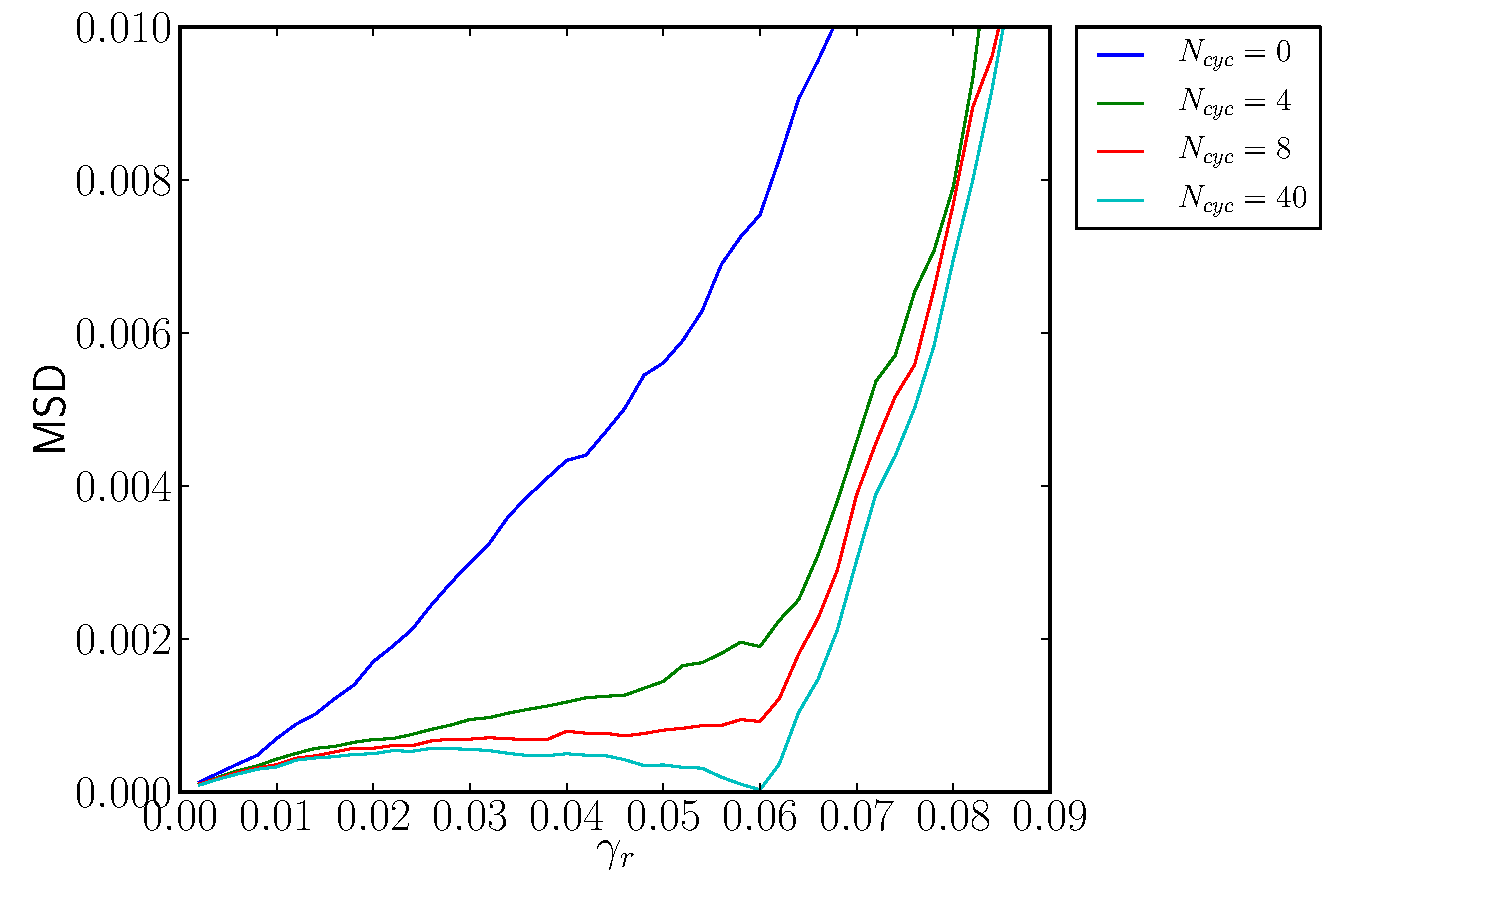
\includegraphics[width=0.8\textwidth]{MemoryKASingle.pdf} 
\caption{Mean squared displacement between configurations before and after a full deformation cycle of amplitude $\gamma_{r}$, for a different number of training cycles of amplitude $\gamma_{1} = 0.06$, as a function of $\gamma_{r}$. Data are relative to initially undeformed KA samples with $N=4000$ and whose effective temperature is $T=0.466$. It's clear how trainings of increasing length produce samples that show a memory of the training amplitude. \label{fig:SingleMemoryLJ}}
\end{figure}

The behavior in \autoref{fig:SingleMemoryLJ} depends on $\gamma_{acc}$:
\begin{itemize}
\item For no training at all ($\gamma_{acc} = 0$), the MSD grows smoothly as $\gamma_{r}$ is increased. This is because a larger $\gamma_{r}$ is related to a larger capability to move away from the initial unstrained configuration (in the language of the mortal random walk in \autoref{sec:DiffusionBehavior}, a larger $\gamma_{r}$ corresponds to a larger $D$ in \autoref{eq:MortalRandomWalkMSD}).
\item For larger values of the training $\gamma_{acc}$ the MSD is lower, and develops a kink in correspondence to a value of $\gamma_{r} = \gamma_{1}$. 
\item For very large values of $\gamma_{acc}$ the MSD plot becomes independent from $\gamma_{acc}$, with a deep dip at $\gamma_{1}$. The independence from $\gamma_{acc}$ is a consequence of the fact that in this case all the samples reach absorbing states, so that a prolongation of the training has no effect on them.
In this case the MSD shown in \autoref{eq:MortalRandomWalkMSD} is zero in correspondence of $\gamma_{1}$ (as it should, because states are absorbing), but has a non-zero value for all the other values of $\gamma_{r}$. This allows us to conclude that, in general, \emph{an absorbing state for an oscillation amplitude $\gamma_{1}$ is not an absorbing state for a $\gamma_{r} \neq \gamma_{1}$}. 
\end{itemize}

These facts clearly show that one can recover the value of the training $\gamma_{1}$ from trained samples simply by performing reading cycles on them, and looking for kinks in the MSD$(\gamma_{r})$ plot.\\
The non-zero MSD for any value of $\gamma_{r}$ but $\gamma_{1}$ in the reading phase has a more subtle implication: the state reached after the reading cycle of amplitude $\gamma_{r}$ does not coincide with the initial one, and this new state doesn't need to be an absorbing state for $\gamma_{1}$. In other words this new state won't necessarily give a zero MSD if re-read at an amplitude $\gamma_{1}$, meaning that memory of the training at $\gamma_{1}$ has been erased. Summarizing, \emph{a single cycle of an amplitude which does not coincide with the training amplitude is able to make the system ``forget'' about the training}. Thus, the reading of memory is an operation that destructs the memory.\\

How does the mechanism of memory erasure in the LJ model work? The answer to this question is rooted in the nature of the absorbing states, and is related to another question: how does an absorbing state actually manage to retain the same state when read with a cycle whose amplitude is equal to its training amplitude ($\gamma_{r} = \gamma_{1}$)? By monitoring the behavior of an absorbing configuration during a reading cycle we notice that an absorbing cycle undergoes several transitions (in the sense defined in \autoref{sec:AQSDynamics}). This is evident, for instance, by looking at the evolution of the positions of the particles in the configuration in space or by monitoring the potential energy $U$ as the strain $\gamma$ is cycled during the reading phase. An animation of the evolution of the positions of the particles can be found online on \cite{mygithub} (see \autoref{app:DataPreservation} for instructions), whereas plots of $U$ during the reading cycle are displayed in \autoref{fig:EnergyVsStrainAbsorbing}.
By looking at the evolution of the system in real space and the behavior of $U$ during a reading cycle, one sees that at some values of the strain the sample undergoes abrupt rearrangements, and that to these correspond discontinuities in the energy. At the end of the full cycle, somewhat surprisingly, the sample returns back to its original state. This is because \emph{the sequence of transitions constitutes a chain of rearrangements that is able to revert the sample to its original state}. It is clear that if such a sequence is altered, for instance by changing the value of the amplitude, the sample is not anymore guaranteed to return to its original state. This is the reason why one gets a non-zero average MSD in \autoref{fig:SingleMemoryLJ}) for $\gamma_{r} \neq \gamma_{1}$. The consequence of this is that the sample is actually kicked out of the absorbing configuration, and thus loses memory of its training.

\begin{landscape}
	\begin{figure}
		\centering
		\begin{subfigure}[b]{0.48\textwidth}
				\centering
				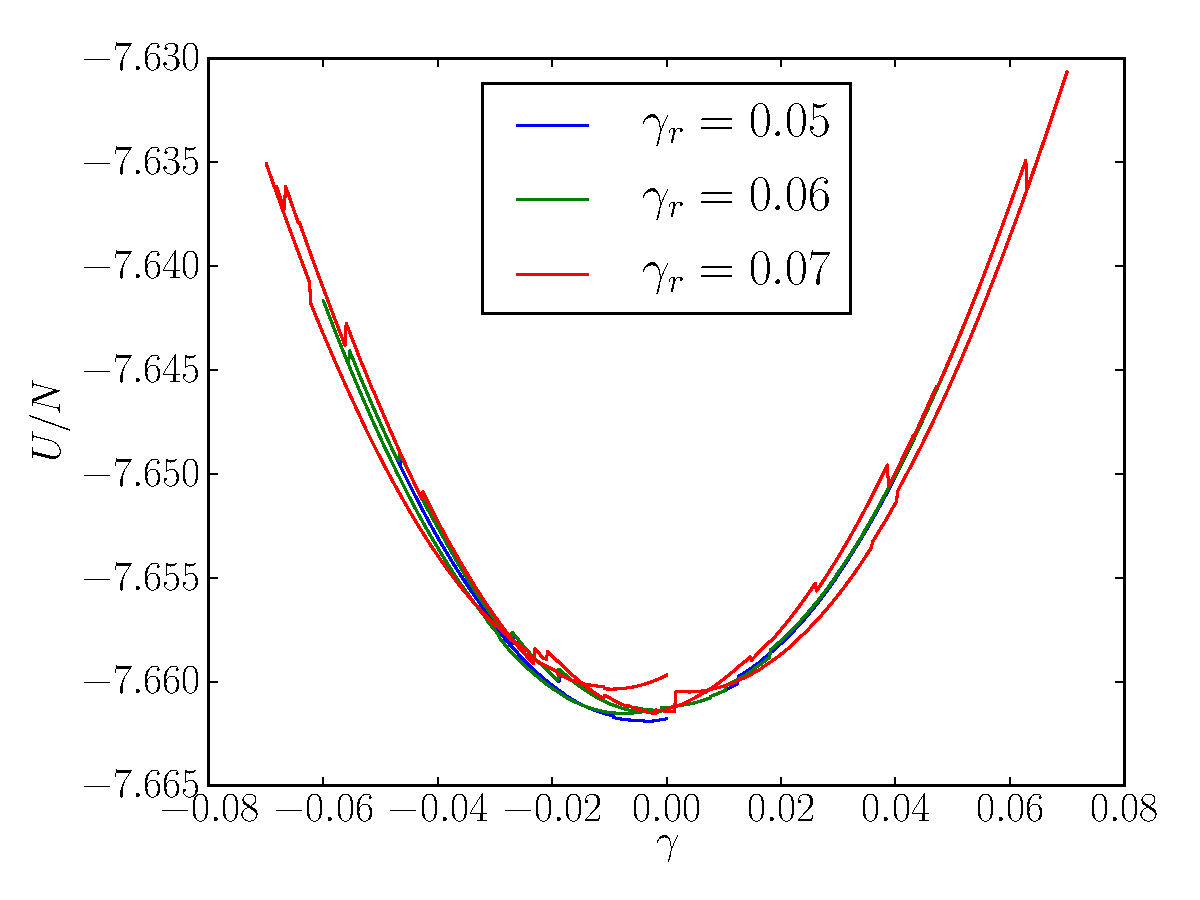
\includegraphics[width = \textwidth]{Ecycle.pdf}
				\caption{\label{fig:UcycleAll}}
		\end{subfigure} 	\\
		\begin{subfigure}[b]{0.48\textwidth}
				\centering
				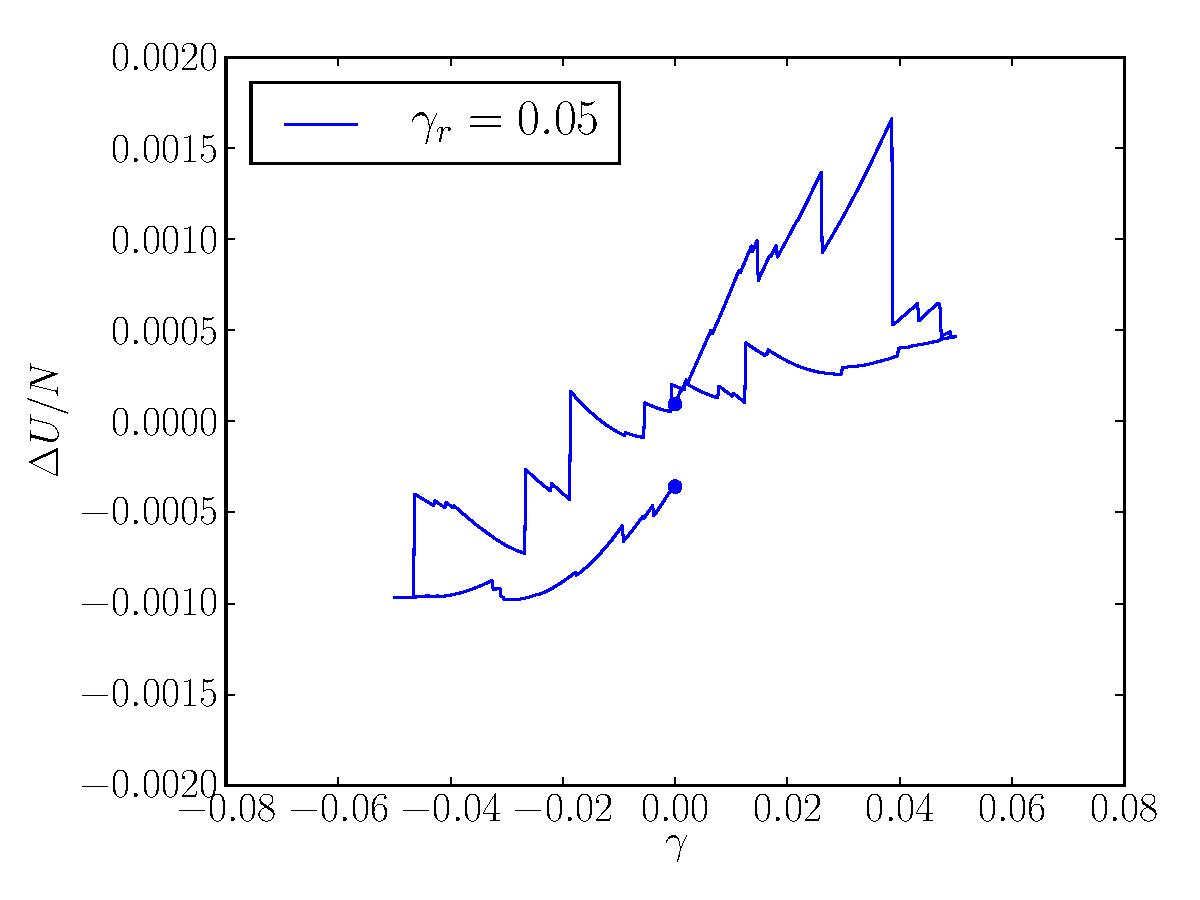
\includegraphics[width = \textwidth]{EcycleUnder.pdf}
				\caption{\label{fig:UcycleUnder}}
		\end{subfigure} 
		\begin{subfigure}[b]{0.48\textwidth}
				\centering
				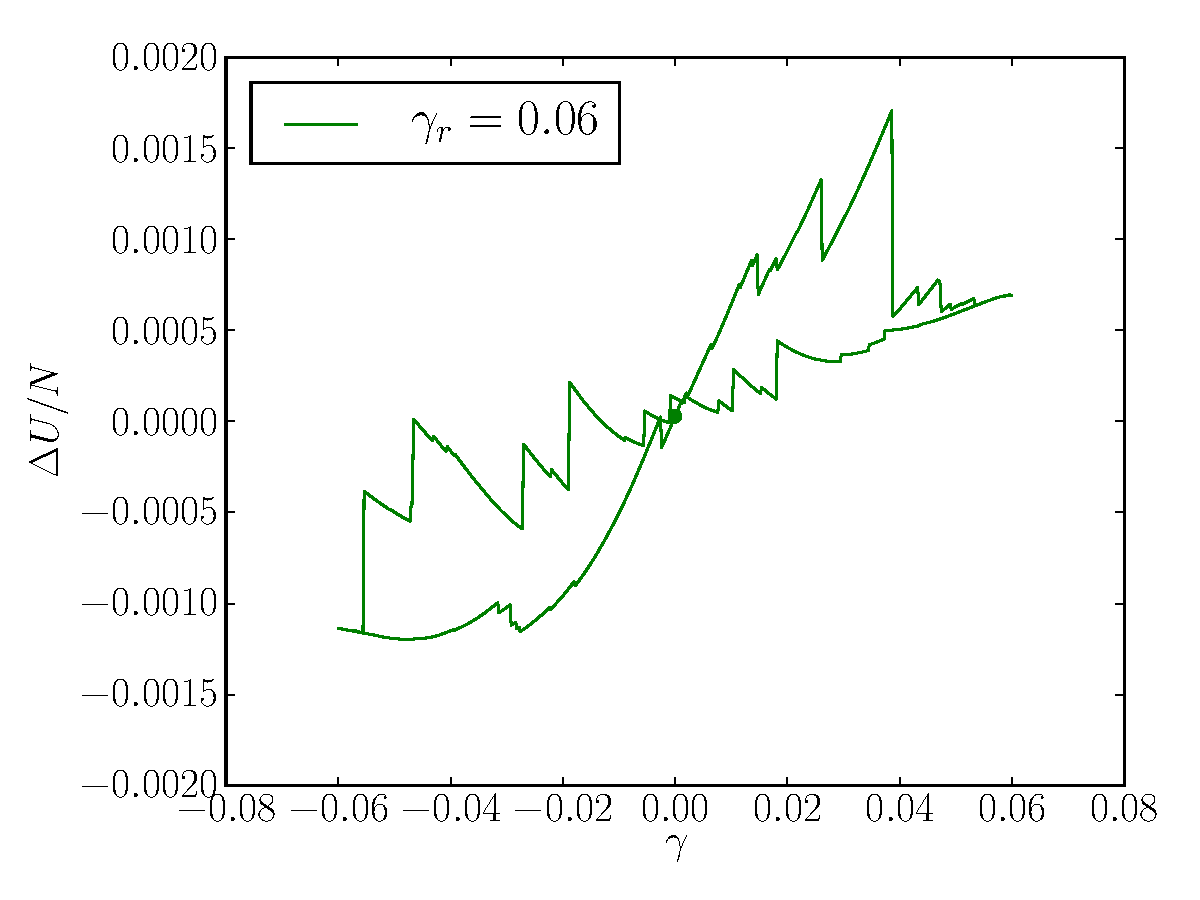
\includegraphics[width = \textwidth]{EcycleEqual.pdf}
				\caption{\label{fig:UcycleEqual}}
		\end{subfigure} 
		\begin{subfigure}[b]{0.48\textwidth}
				\centering
				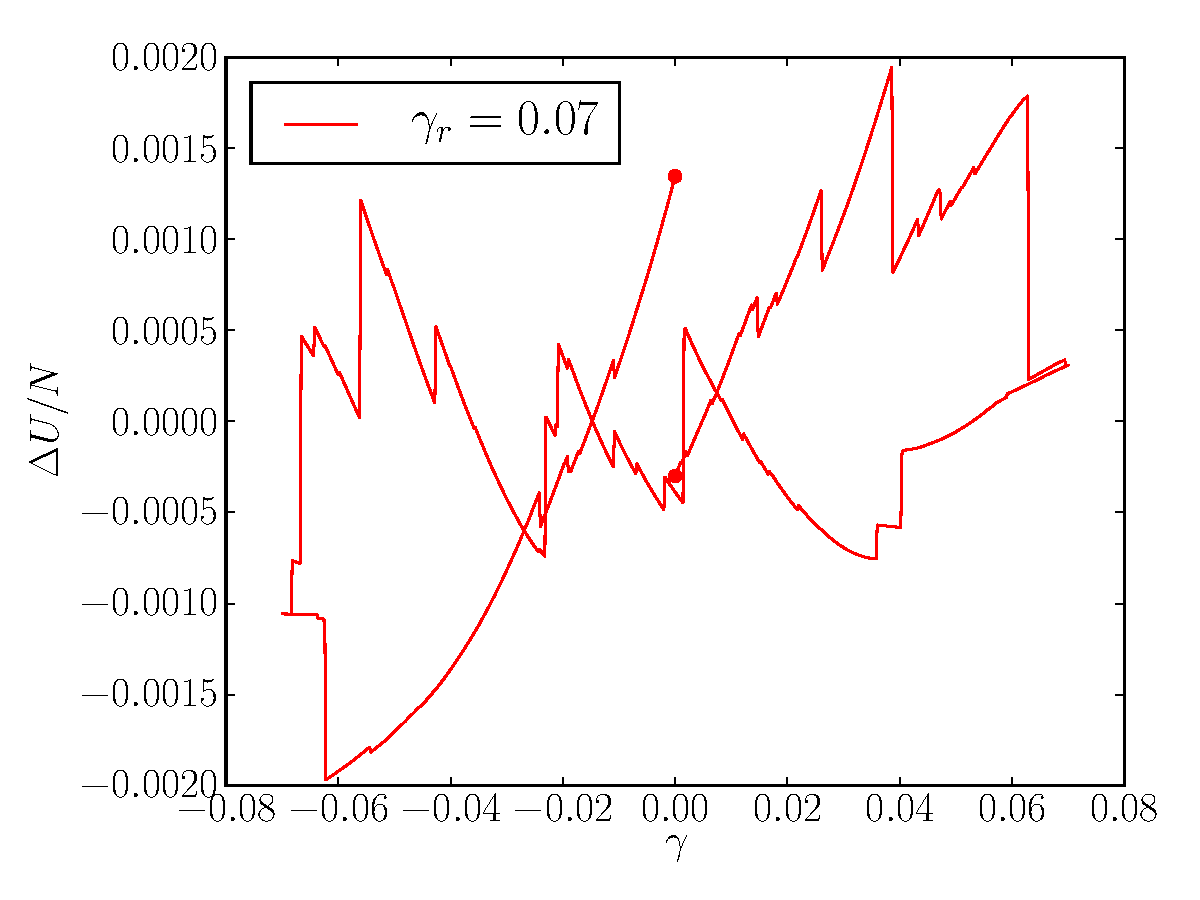
\includegraphics[width = \textwidth]{EcycleOver.pdf}
				\caption{\label{fig:UcycleOver}}
		\end{subfigure} 
	\caption{
	Energy per particle as a function of the strain $\gamma$ for a sample of $N=4000$ trained at $\gamma_{1} = 0.06$ and performing a single cycle of amplitude $\gamma_{r} = 0.05, 0.06, 0.07$ (in blue, green, red respectively).
	In (\subref{fig:UcycleAll}), all the curves overlap and can be approximated by a quadratic function. In (\subref{fig:UcycleUnder}), (\subref{fig:UcycleEqual}), (\subref{fig:UcycleOver}), the quadratic background is subtracted. The initial sample is in an absorbing state for amplitudes of $\gamma_{max} = 0.06$, so in (\subref{fig:UcycleEqual}) the endpoints of the curve meet at $\gamma = 0$. This is not the case for (\subref{fig:UcycleUnder}) and (\subref{fig:UcycleOver}), where cycles of amplitudes $\gamma_{r} = 0.05$ and $0.07$ respectively are performed.  
	\label{fig:EnergyVsStrainAbsorbing}}
	\end{figure}
\end{landscape}

\subsubsection{Single memory in the NK model}

We perform a training and reading on NK configurations as well, in a way that mirrors that followed in the LJ case. We choose $N = 20$, $K = 10$, averaging on $\approx 8$ inherent configurations for $\approx 200$ instances of the couplings $a$, $b$ and $J$, setting $\gamma_{1} = 0.3$ and performing trainings of different durations. The measure of the displacement in the reading phase is given by the Hamming distance in \autoref{eq:HammingDistance} between the configuration before and after the read. Results are plotted in \autoref{fig:SingleMemoryNK}, and are in qualitative agreement with what is observed in the LJ case: the possibility to encode, read and erase memory thus exists in the NK model as well. 

\begin{figure} 
\centering 
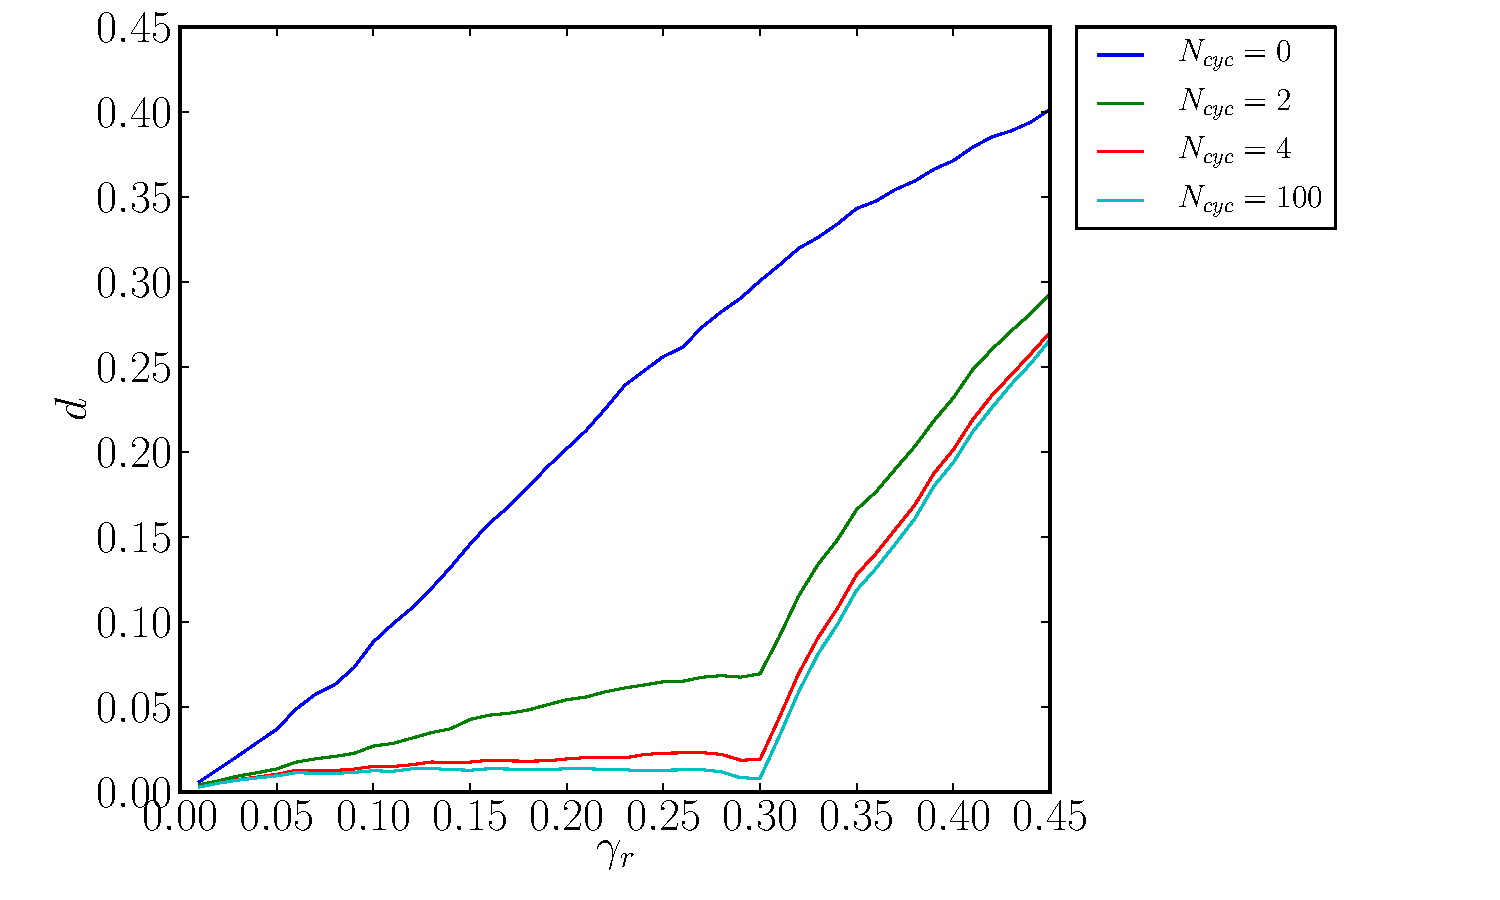
\includegraphics[width=0.8\textwidth]{MemoryNKSingle.pdf} 
\caption{Hamming distance between configurations before and after a full deformation cycle of amplitude $\gamma_{r}$, for a different number of training cycles of amplitude $\gamma_{1} = 0.3$, as a function of $\gamma_{r}$. Data are relative to initially undeformed NK samples with $N=20$ and whose effective temperature is $T=1.0$. It's clear how trainings of increasing length yield samples that show a memory of the training amplitude. \label{fig:SingleMemoryNK}}
\end{figure}

\subsubsection{Single memory in the TM model}

One can probe for memory effects in the TM model, but the procedure is fairly different with respect to that followed in the LJ and NK cases. 
First of all, to do so we generate $P$ matrices for different values of $\gamma_{max}$, following the procedure described in \autoref{app:TMDetails}.
Once a $\gamma_{1}$ is chosen, we consider the configurations trained by $N_{cyc}$ oscillations (equivalent to $\gamma_{acc} = 4\gamma_{1} N_{cyc}$). These are those with the same index of the non-empty rows of the matrix $P_{\gamma_{1}}^{N_{cyc}}$, where $P_{\gamma_{1}}$ is the matrix associated to the deformation up to $\gamma_{1}$. This is because $P_{\gamma_{1}}^{N_{cyc}}$ is the matrix that maps any of the states of the undeformed landscape into those that are reached by them after $N_{cyc}$ oscillations. We call to the set of such states $A_{N_{cyc}}$.
To probe the behavior of such states under a single reading cycle of amplitude $\gamma_{r}$, we check whether they are absorbing cycles for $\gamma_{r}$, i.e. we verify if the condition $P_{\gamma_{r}} \mathbf{R} = \mathbf{R}$ is satisfied, for each $\mathbf{R}$ state in $A_{N_{cyc}}$. The validity of this condition is easy to check, because it holds true if and only if the matrix element on the diagonal of $P_{\gamma_{r}}$ corresponding to such states is equal to one. In \autoref{fig:SingleMemoryTM} we plot the fraction of non-absorbing states (i.e. $\mathbf{R}$ states in $A_{N_{cyc}}$ that don't meet the condition $P_{\gamma_{r}} \mathbf{R} = \mathbf{R}$) for different values of $\gamma_{r}$, obtained by studying the states belonging to a space with $M= 10000$ structures with probability $\tau = 0.04$ to be destabilized and ``trained'' by a different number of cycles of amplitude $\gamma_{1} = 60$.

\begin{figure} 
\centering 
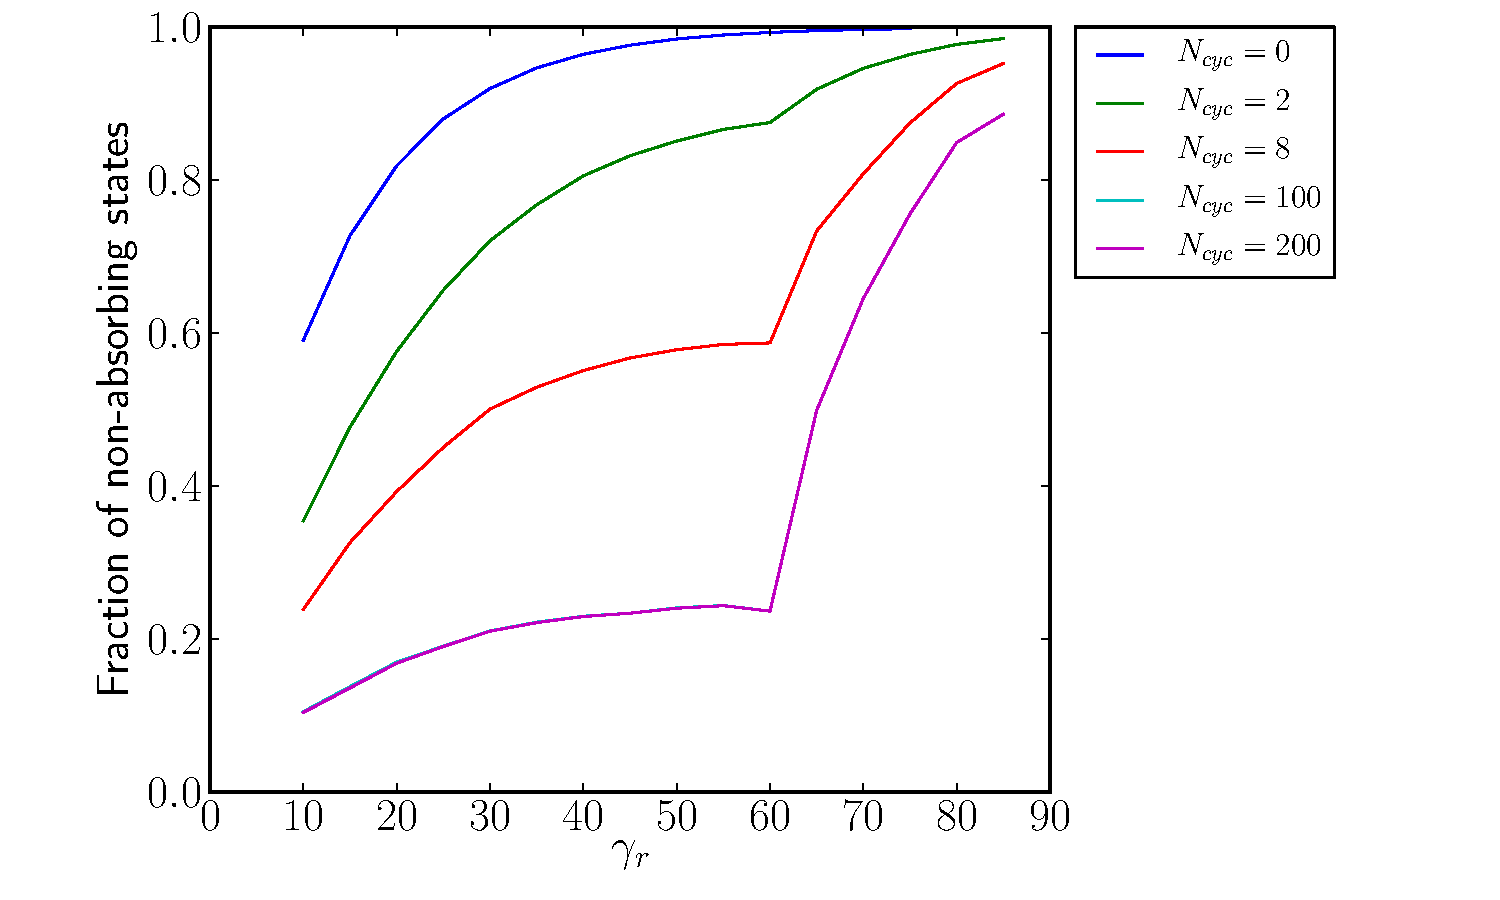
\includegraphics[width=0.8\textwidth]{MemoryTMSingle.pdf} 
\caption{Fraction of inherent states that are not invariant under the application of a $P_{\gamma_{r}}$, starting from a pool of states trained by a different number of applications of the matrix $P_{\gamma_{1}}$ with $\gamma_{1} = 60$, as a function of $\gamma_{r}$. Data are obtained within the TM model setting $M=10000$. It's clear how trainings of increasing length yield samples that show a memory of the training amplitude. \label{fig:SingleMemoryTM}}
\end{figure}

Strictly speaking, the plot in \autoref{fig:SingleMemoryTM} is not equivalent to those in \autoref{fig:SingleMemoryLJ} and \autoref{fig:SingleMemoryNK}. In the LJ and NK models a notion of distance exists between configurations, so that one is able to quantify the displacement experienced by the samples during the reading phase (using the MSD and the Hamming distance respectively). Such information is not given by the TM model, which however delivers a very similar information: it tells whether states are left unchanged or are modified by a reading cycle of amplitude $\gamma_{r}$\footnote{In this sense, the TM model gives a ``yes or no'' information about whether a sample is changed by a reading cycle; the LJ and NK models do more: they give a measure of \emph{how much} a sample is affected by a reading cycle.}.

\subsection{Multiple memories}

The training can be modified so that it consists in the alternated repetition of cycles of amplitude $\gamma_{1}$ and $\gamma_{2}$, like in \autoref{fig:DoubleTriangleWave}. The rationale behind this protocol is to encode \emph{multiple} memories in our samples, and be able to read the values of the different training amplitudes in the reading phase.
\begin{figure} 
\centering 
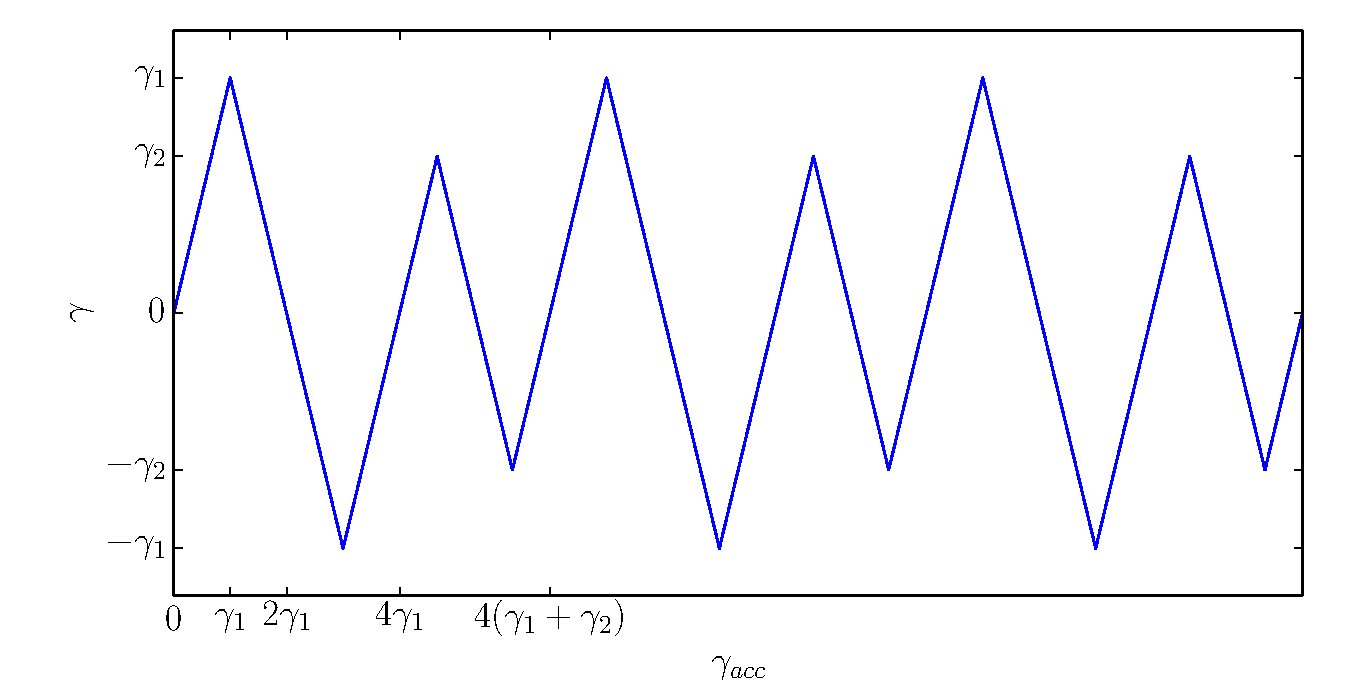
\includegraphics[width=0.8\textwidth]{TriangleDouble.pdf} 
\caption{Strain profile applied to a sample to encode a double memory.\label{fig:DoubleTriangleWave}}
\end{figure}
The cycles in $\gamma$ have the form $0 \rightarrow \gamma_{1} \rightarrow 0 \rightarrow  -\gamma_{1} \rightarrow 0 \rightarrow \gamma_{2} \rightarrow 0 \rightarrow  -\gamma_{2} \rightarrow 0$. 
We repeat such cycle $N_{cyc}$ times, so that after the training the sample as been subjected to an accumulated strain $\gamma_{acc} = 4(\gamma_{1} + \gamma_{2})N_{cyc}$. This can be straightforwardly done in the LJ and NK cases, whereas (as described above in the case of single memory), a different scheme must be adopted with the TM model. \\
For what concerns the LJ model, we choose $\gamma_{1} = 0.06$ and $\gamma_{2} = 0.04$ and train samples of the same size and initial effective temperature as those trained with a single amplitude by performing $N_{cyc}$ on them. We then take copies of the trained samples and subject them to a reading cycle of amplitude $\gamma_{r}$. As above we measure the MSD of the configurations as a function of $\gamma_{r}$. As it can be seen from \autoref{fig:DoubleMemoryLJ}, the MSD has two kinks in correspondence of $\gamma_{1}$ and $\gamma_{2}$, which are both visible for sufficiently high $N_{cyc}$. In addition, for a high number of $N_{cyc}$, the MSD curve converges to a curve showing clearly the trace of the two training amplitudes. By looking at the data, it's reasonable to assume that this will be true for an arbitrarily large number of $N_{cyc}$, so that the two memories will be \emph{persistent} for $\gamma_{acc} \rightarrow \infty$.

\begin{figure} 
\centering 
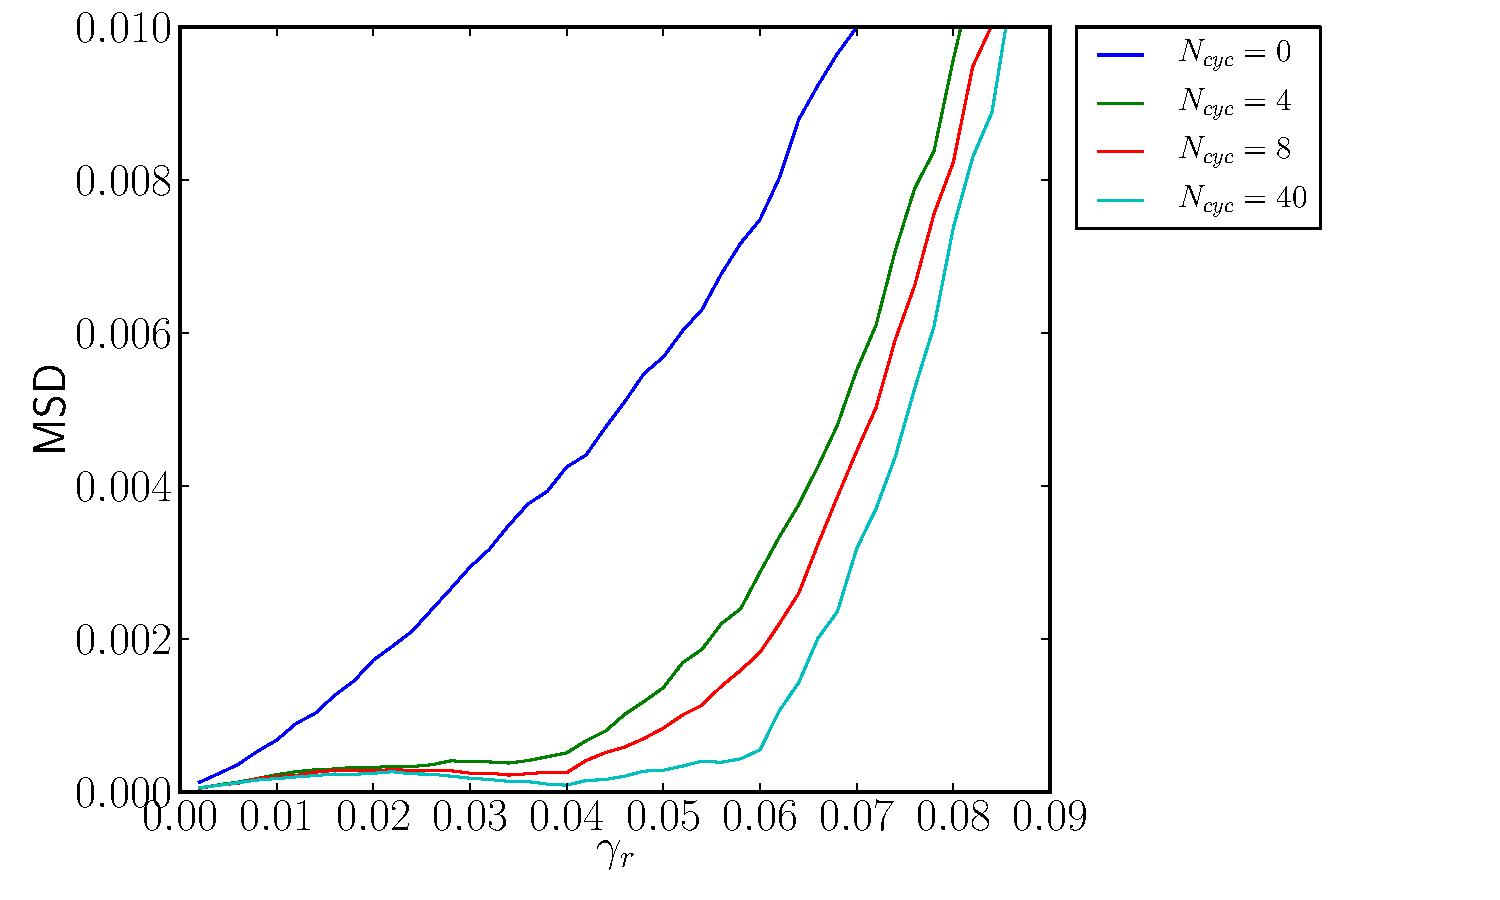
\includegraphics[width=0.8\textwidth]{MemoryKADouble.pdf} 
\caption{Mean squared displacement between configurations before and after a full deformation cycle of amplitude $\gamma_{r}$, for a different number of training cycles alternating training amplitudes $\gamma_{1} = 0.06$ and $\gamma_{1} = 0.04$, as a function of $\gamma_{r}$. Data are relative to initially undeformed KA samples with $N=4000$ and whose effective temperature is $T=0.466$. In the case of the longest trainings samples show a memory of both the training amplitudes. \label{fig:DoubleMemoryLJ}}
\end{figure}
In the NK case, we choose $\gamma_{1} = 0.06$ and $\gamma_{2} = 0.04$ and train the samples for different $N_{cyc}$ with the same $N$, $K$, initial effective temperature and values of the couplings of those trained with a single amplitude. Again, we use the Hamming distance $d$ as a measure of the change in configurations in the reading phase and plot $d$ for different values of $\gamma_{r}$ in \autoref{fig:DoubleMemoryNK}. As in the LJ case, the training amplitudes can be read by looking at kinks (discontinuities in the first derivative) in the plot, and again they appear persistent in the limit $\gamma_{acc} \rightarrow \infty$.

\begin{figure} 
\centering 
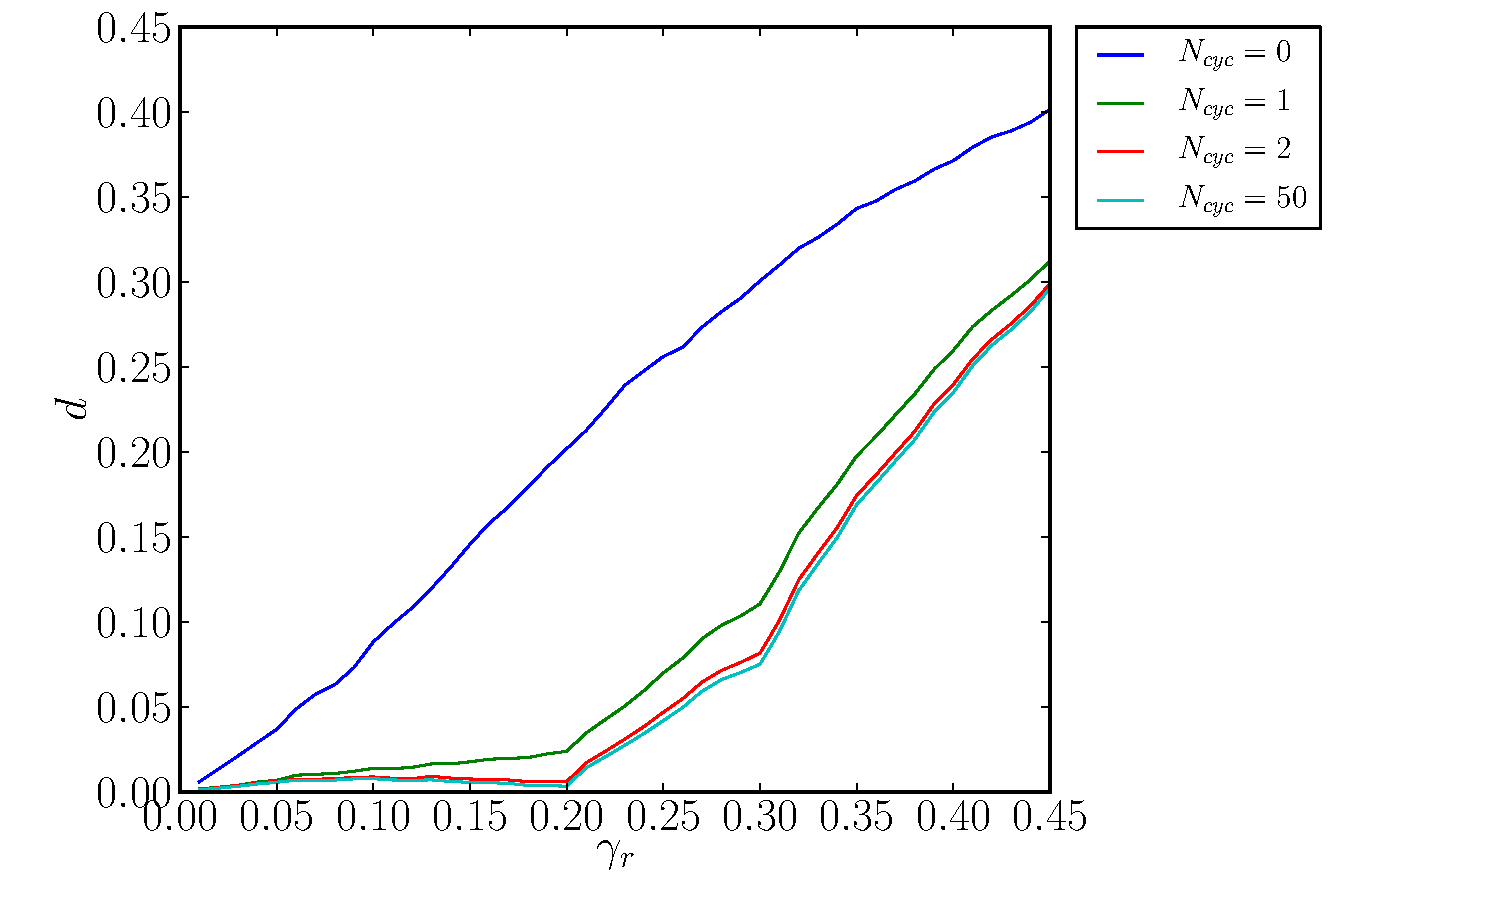
\includegraphics[width=0.8\textwidth]{MemoryNKDouble.pdf} 
\caption{Hamming distance between between configurations before and after a full deformation cycle of amplitude $\gamma_{r}$, for a different number of training cycles alternating training amplitudes $\gamma_{1} = 0.3$ and $\gamma_{1} = 0.2$, as a function of $\gamma_{r}$. Data are relative to initially undeformed NK samples with $N=20$ and whose effective temperature is $T=1.0$. In the case of the longest trainings samples show a memory of both the training amplitudes. \label{fig:DoubleMemoryNK}}
\end{figure}

In the case of the TM model the ``trained'' configurations are those with the same index of the non-empty rows of the matrix $(P_{\gamma_{2}} P_{\gamma_{1}})^{N_{cyc}}$, where $P_{\gamma_{1}}$ and $P_{\gamma_{2}}$ are the matrices associated to the deformation up to $\gamma_{1}$ and $\gamma_{2}$. We refer to the set of such states as $B_{N_{cyc}}$. Exactly as in the reading of single memories, we compute the fraction of non-absorbing states (i.e. states in $B_{N_{cyc}}$ that don't meet the condition $P_{\gamma_{r}} \mathbf{R} = \mathbf{R}$) for different values of $\gamma_{r}$) as a function of $\gamma_{max}$.
From the analysis of \autoref{fig:DoubleMemoryTM}, it is clear that a double memory can be encoded in an ensemble of structures in the TM model.

\begin{figure} 
\centering 
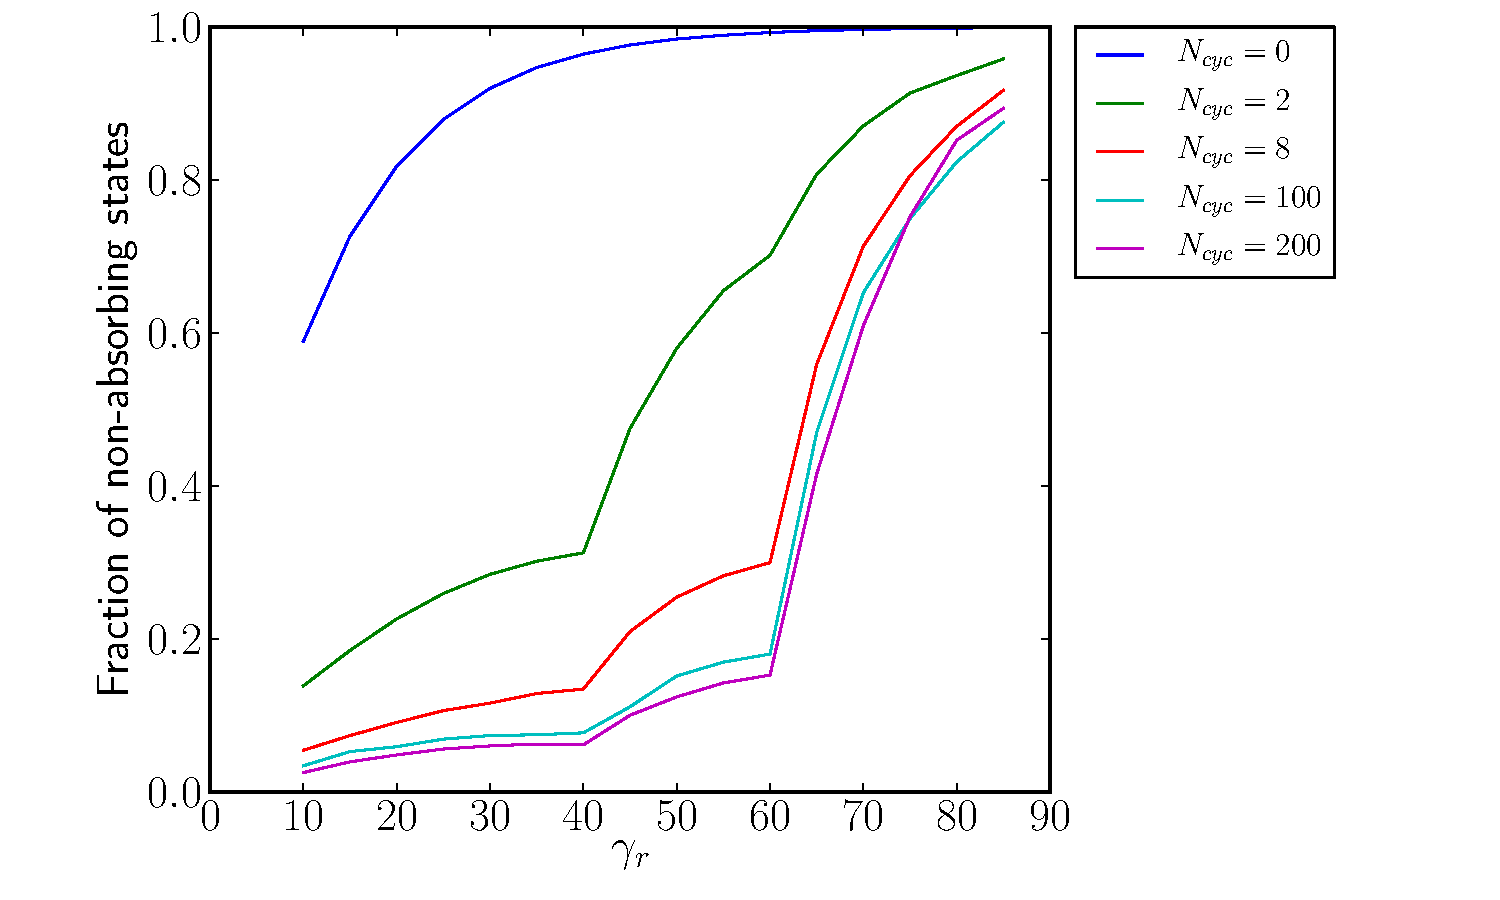
\includegraphics[width=0.8\textwidth]{MemoryTMDouble.pdf} 
\caption{Fraction of inherent states that are not invariant under the application of a $P_{\gamma_{r}}$, starting from a pool of states trained by a different number of applications of the matrix $P_{\gamma_{1}}$ with $\gamma_{1} = 60$ and of $P_{\gamma_{2}}$ with $\gamma_{2} = 40$, as a function of $\gamma_{r}$. Data are obtained within the TM model setting $M=10000$. It's clear how trainings of increasing $N_{cyc}$ produce samples that show a memory of the training amplitudes. \label{fig:DoubleMemoryTM}}
\end{figure}

\subsection{Summary and comparison with colloidal suspensions}

In this chapter we have verified that it is indeed possible to encode in our systems single and double memories using the same protocol adopted in \cite{keim2011generic} in the case of noncolloidal suspensions. In fact, this can be achieved by training our samples with shear deformation cycles of a given amplitude and by deforming them alternating two different oscillation amplitudes respectively. This is evident, for instance, from the analysis of \autoref{fig:SingleMemoryLJ} and \autoref{fig:DoubleMemoryLJ}.\\
However, we found that LJ and NK models show an important difference with the memory behavior of noncolloidal suspensions. In these two classes of systems absorbing states for a given amplitude can be destabilized by shear deformation cycles of a lesser amplitude. This fact is related to the nature of absorbing states in the LJ and NK models. An absorbing state is such because during a deformation cycle of amplitude $\gamma_{1}$ the system undergoes various rearrangements during a cycle, and the full sequence of them has the effect of bringing the system to the state occupied before the application of the deformation cycle (\autoref{fig:EnergyVsStrainAbsorbing}). If the deformation amplitude is changed, such sequence of rearrangements is altered, and the system can fail to come back to its initial state. 
We showed that this fact has the consequence that multiple memories can stay encoded in LJ and NK systems even if these are subjected to indefinitely long series of training cycles. This is because in long trainings different training amplitudes ``compete'' with the each other. In particular, the action of small amplitudes is that of partially erasing the effect of larger amplitudes, so that samples never get ``completely trained'' and no amplitude takes over the others. As it can be checked by comparing \autoref{fig:SingleMemoryLJ} and \autoref{fig:DoubleMemoryLJ} with \autoref{fig:SuspensionMemory}, this is different from what happens in noncolloidal suspensions without noise, and mirrors what is observed in models of the same suspensions when noise is added \cite{keim2011generic}.
The effect of memory erasure due to reading at an amplitude other than the training one makes reading a \emph{destructive} operation.
However, it is possible to devise a protocol that can overcome the erasure of memory due to the reading operation in our systems: given an ensemble of systems trained in the same way, one can read the information encoded in them by performing on each of the samples a single deformation cycle, with a reading amplitude which is different for each system. Such reading operation is destructive at the level of the memory in a single sample, but allows to retrieve the desired information from the ensemble. Once that the information has been obtained, all the samples of the ensemble can be ``retrained'' using such information, so to restore in them the original information.

We surmise that the observations in this chapter hold true for LJ and NK systems with much larger $N$. We expect this because the transition at $\gamma_{c}$ in \autoref{ch:ParticleModelsResults} is likely to exist in the thermodynamic limit, as well as the mechanism of destabilization of absorbing states as the amplitude of deformation is changed. \\
Furthermore, the observation of single and double memories in the TM model strengthens the idea that memory phenomena are indeed a general feature of the athermal dynamics of oscillatory deformed LJ and NK systems.
